\documentclass{beamer}

% Most of the preamble is in here.
\usepackage{iansslides}

\begin{document}


\section{The Counting Numbers}


\begin{frame}
  \begin{columns}
    \begin{column}{0.3\textwidth}
      \centering
      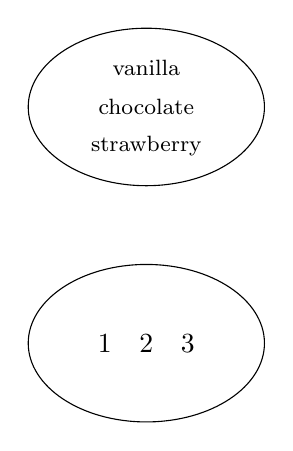
\begin{tikzpicture}
        \draw (0,0) ellipse (1.5 and 1);
        \draw (0,3) ellipse (1.5 and 1);
        \node () at (0,3.5) {\footnotesize vanilla};
        \node () at (0,3) {\footnotesize chocolate};
        \node () at (0,2.5) {\footnotesize strawberry};
        \node (A) at (0,0) {$1 \quad  2 \quad  3$};
      \end{tikzpicture}
    \end{column}
    {\color{gmitgrey!30}\vrule{}} \hspace{0.1\textwidth}
    \begin{column}{0.5\textwidth}
      $\mathbb{N} = \{1,2,3,\ldots\}$ \\[8mm]
      $1 \leftrightarrow $ vanilla \\[8mm]
      $2 \leftrightarrow $ chocolate \\[8mm]
      $3 \leftrightarrow $ strawberry \\[8mm]
    \end{column}
  \end{columns}
\end{frame}


\begin{frame}
  \begin{columns}
    \begin{column}{0.3\textwidth}
      \color{gmitblue} \fontsize{30}{10}
      \[2\mathbb{N}\]
    \end{column}
    {\color{gmitgrey!30}\vrule{}} \hspace{0.1\textwidth}
    \begin{column}{0.5\textwidth}
      $\mathbb{N} = \{1,2,3,\ldots\}$ \\[4mm]
      $2\mathbb{N} = \{2,4,6,\ldots\}$ \\[4mm]
      $\mathbb{N} \leftrightarrow 2 \mathbb{N}$ \\[8mm]
      $1 \leftrightarrow 2$ \\[4mm]
      $2 \leftrightarrow 4$ \\[4mm]
      $3 \leftrightarrow 6$ \\[4mm]
      $\ldots$ \\[4mm]
    \end{column}
  \end{columns}
\end{frame}


\begin{frame}[standout]
  \begin{quote}
    Computer programs are binary strings. \\[8mm]
    Treat them as integers. \\[8mm]
    They're countable. \\[8mm]
    (Slight issue with leading zeros.)
  \end{quote}
\end{frame}


\end{document}